\chapter{Other Measurements Using \Dressed Electrons}
\label{app:dressed_measurements}

\section{Uncertainty Figures}

The values of the various uncertainty in each \phistar bin are presented in the
figures that follow. Figure~\ref{fig:sys_uncert_norm} shows the fractional
uncertainty in the normalized \phistar cross section in data unfolded with
\MADGRAPH while \FIG~\ref{fig:sys_uncert_norm_powheg} shows the fractional
uncertainty in the data unfolded with \POWHEG. The uncertainty on the
normalized \phistar cross section in \MADGRAPH and \POWHEG are shown in
\FIGS~\ref{fig:madgraph_uncert_norm} and \ref{fig:powheg_uncert_norm},
respectively. All of these values are presented in tables in
\APP~\ref{app:uncertainty_tables}.

% Absolute

% fig:sys_uncert_abs
\begin{figure}[!p]
    \centering
    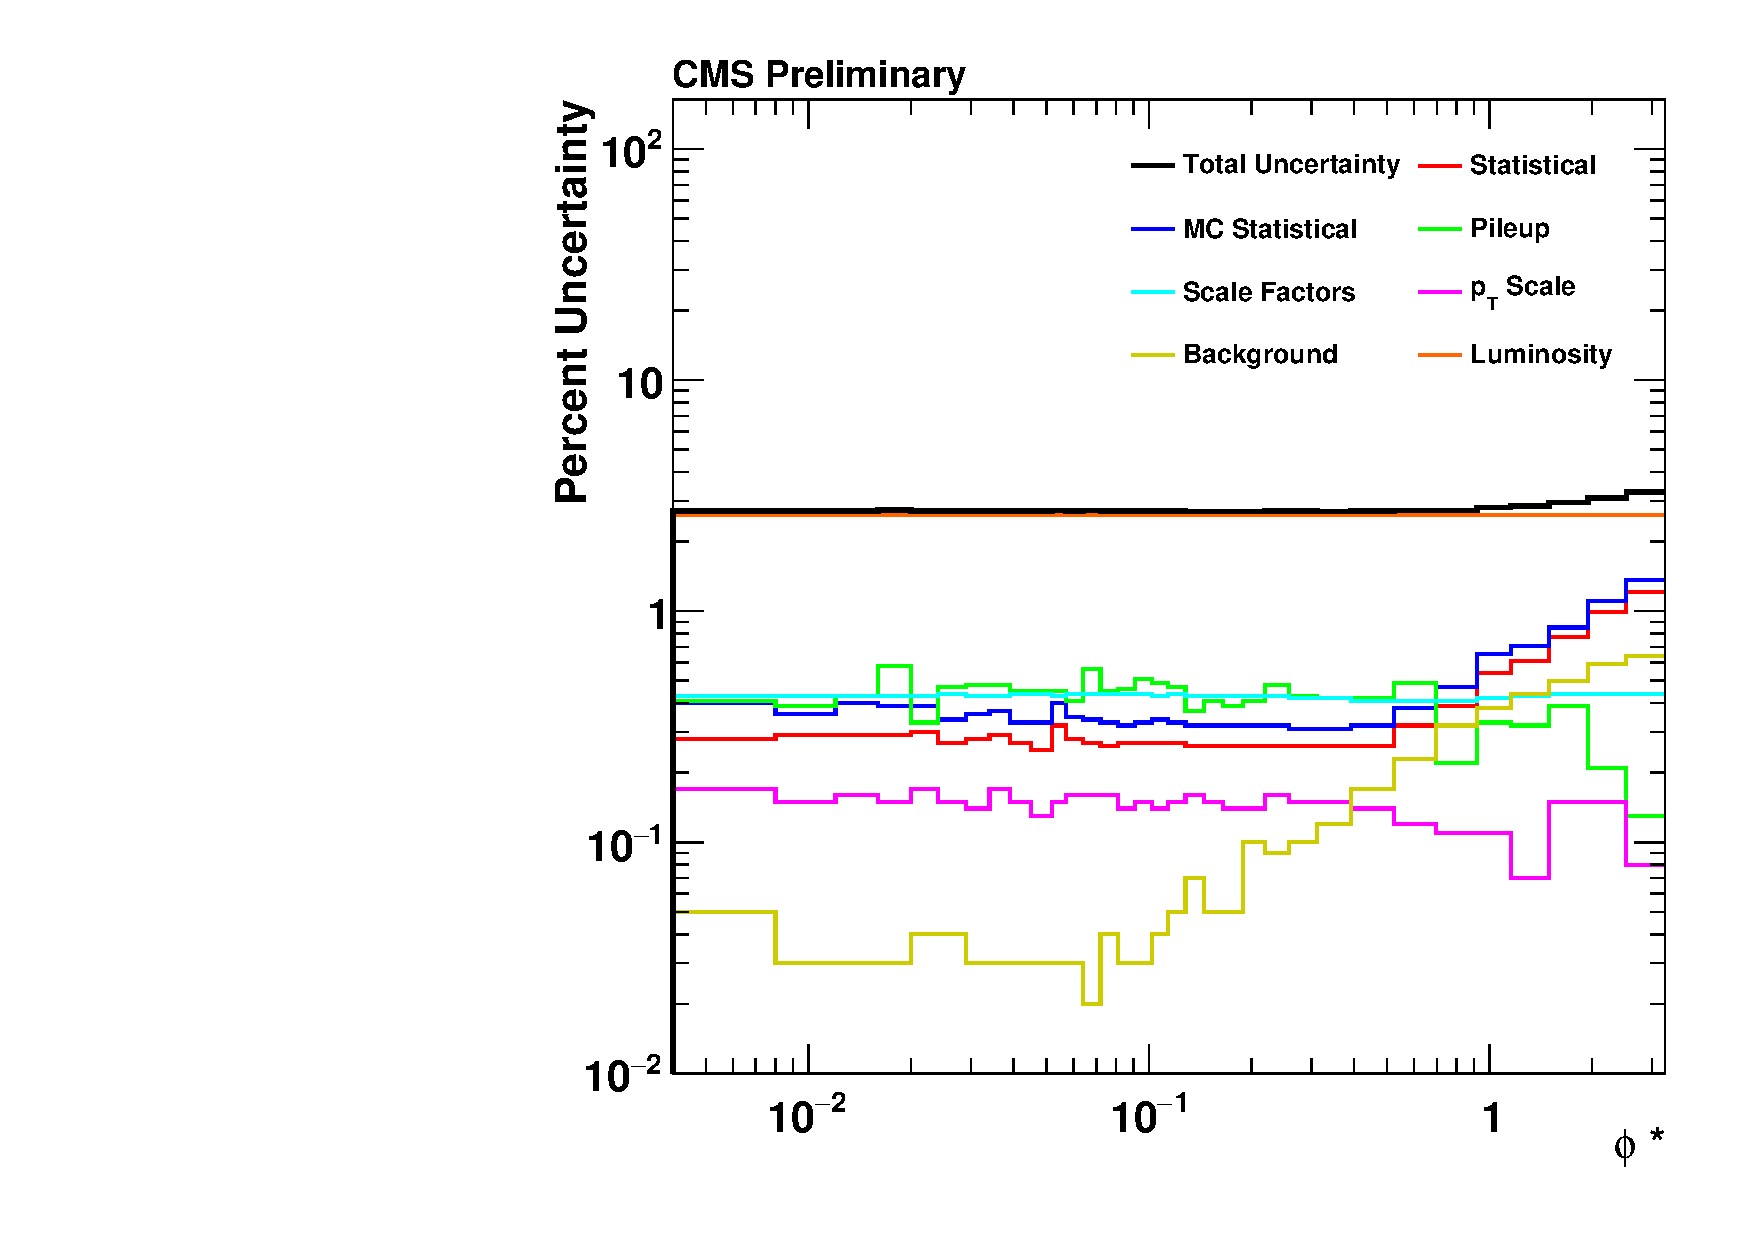
\includegraphics[width=\textwidth]{figures/data_uncertainty_absolute.pdf}
    \caption[
        Fractional errors (in \%) for the absolute cross section measurement
        made with data unfolded with \MADGRAPH.
    ]{
        Fractional errors (in \%) for the absolute cross section measurement
        made with data unfolded with \MADGRAPH. The total value is the sum in
        quadrature of all the other values. These uncertainties are also
        presented in tabular form in \cref{tab:sys_uncert_abs}.
    }
    \label{fig:sys_uncert_abs}
\end{figure}


% fig:sys_uncert_abs_powheg
\begin{figure}[!p]
    \centering
    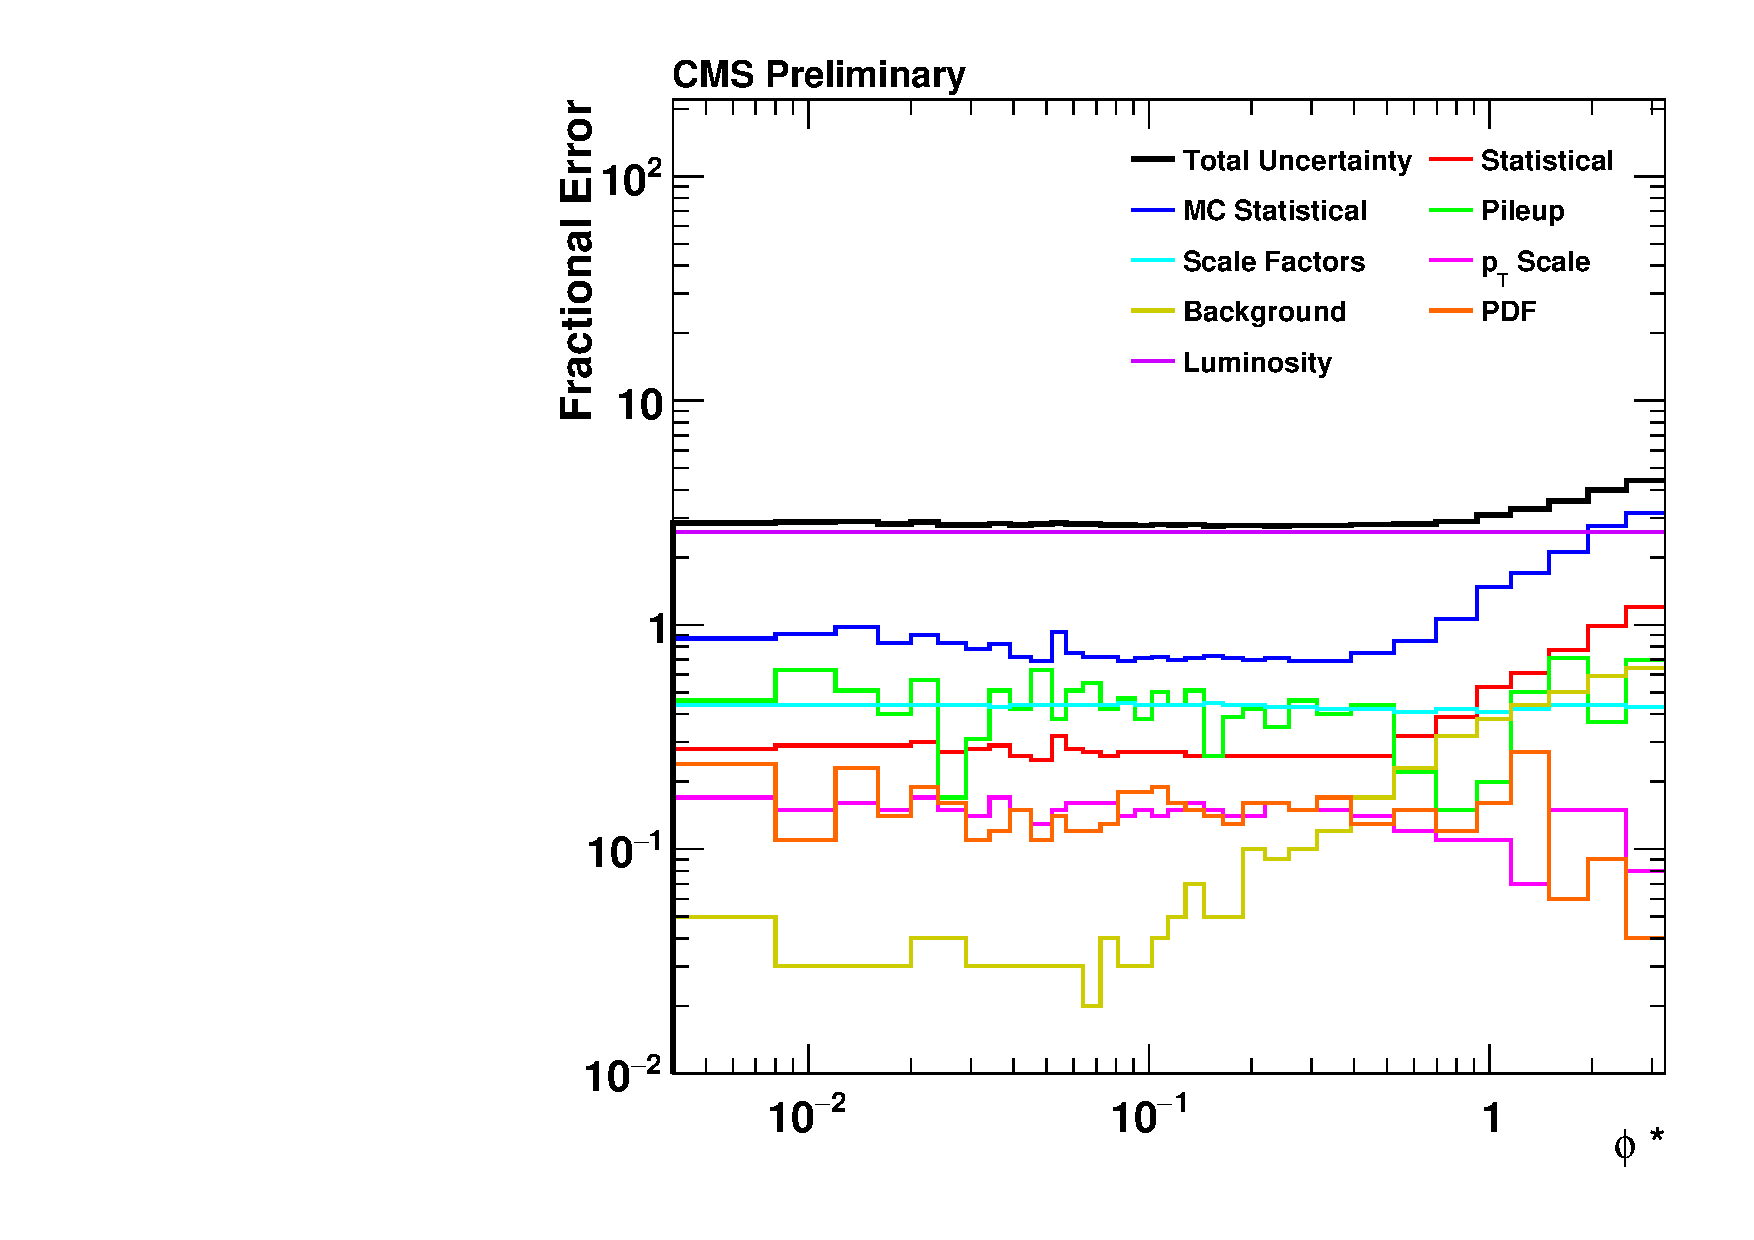
\includegraphics[width=\textwidth]{figures/data_uncertainty_absolute_powheg_unfolded.pdf}
    \caption[
        Fractional errors (in \%) for the absolute cross section measurement
        made with data unfolded with \POWHEG.
    ]{
        Fractional errors (in \%) for the absolute cross section measurement
        made with data unfolded with \POWHEG. The total value is the sum in
        quadrature of all the other values. These uncertainties are also
        presented in tabular form in \cref{tab:sys_uncert_abs_powheg}.
    }
    \label{fig:sys_uncert_abs_powheg}
\end{figure}


% fig:madgraph_uncert_abs
\begin{figure}[!htbp]
    \centering
    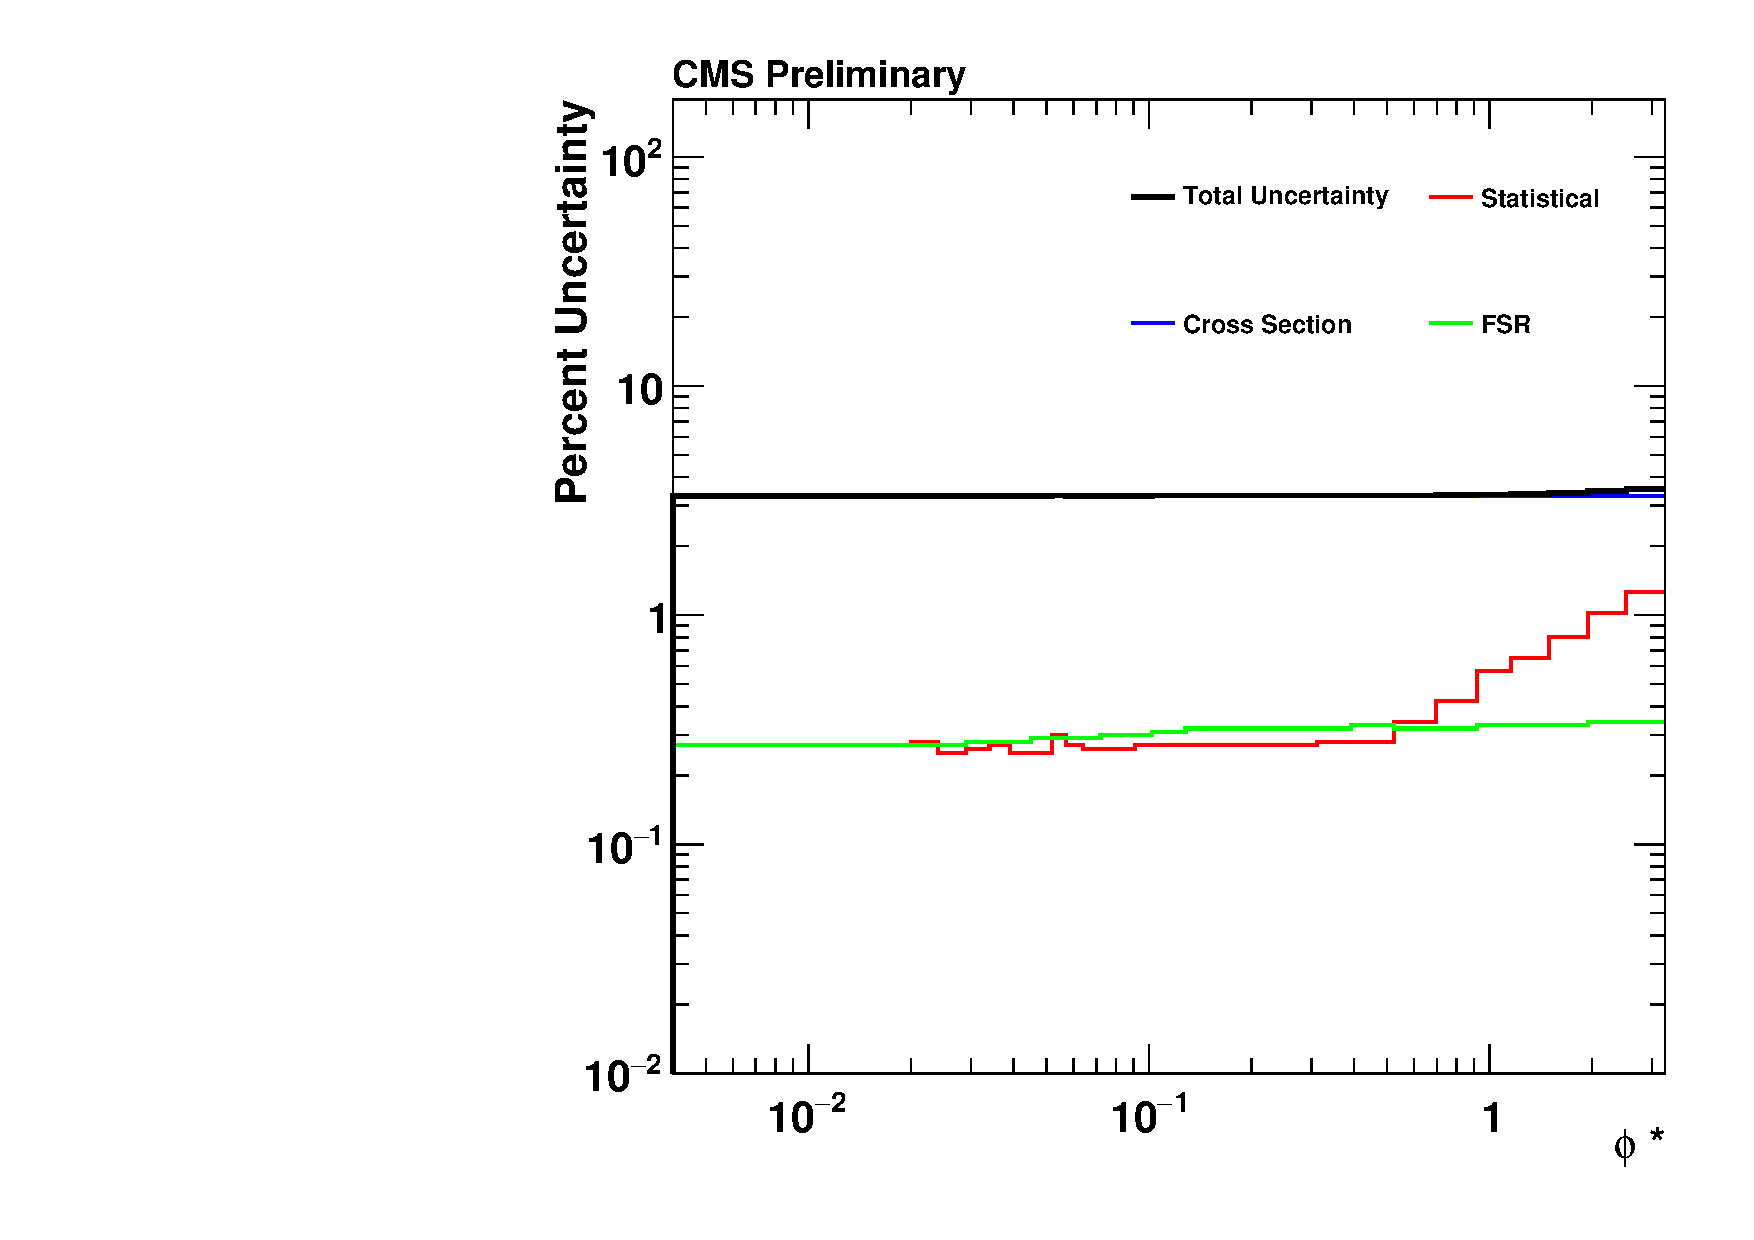
\includegraphics[width=\textwidth]{figures/madgraph_uncertainty_absolute.pdf}
    \caption[
        Fractional errors (in \%) for the absolute cross section from the
        \MADGRAPH MC sample.
    ]{
        Fractional errors (in \%) for the absolute cross section from the
        \MADGRAPH MC sample. These uncertainties are also presented in tabular
        form in \TAB~\ref{tab:madgraph_uncert_abs}.
    }
    \label{fig:madgraph_uncert_abs}
\end{figure}


% fig:powheg_uncert_abs
\begin{figure}[!p]
    \centering
    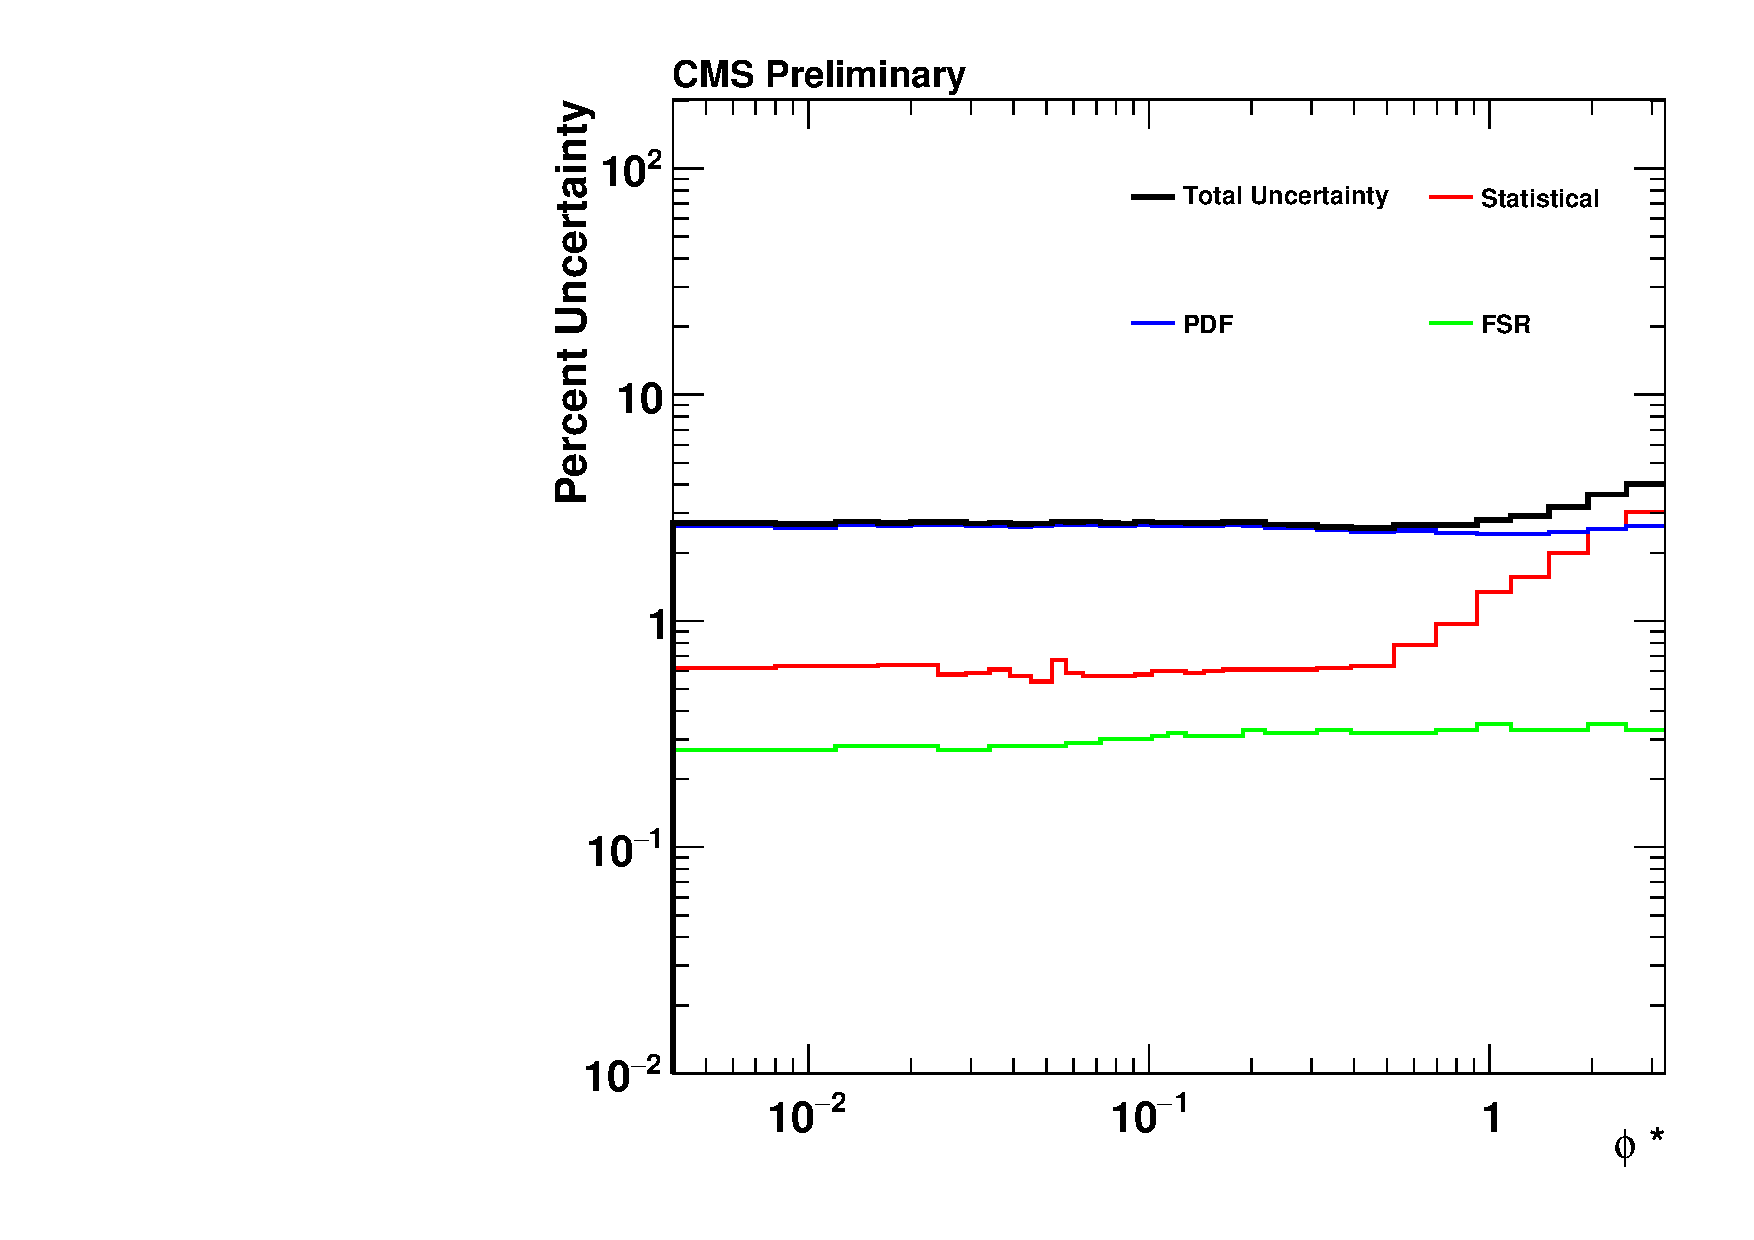
\includegraphics[width=\textwidth]{figures/powheg_uncertainty_absolute.pdf}
    \caption[
        The uncertainties for the absolute cross section from the \POWHEG MC
        sample.
    ]{
        The uncertainties (in \%) for the absolute cross section from the
        \POWHEG MC sample. These uncertainties are also presented in tabular
        form in \cref{tab:powheg_uncert_abs}.
    }
    \label{fig:powheg_uncert_abs}
\end{figure}



\section{Absolute Differential Cross Section}
\label{sec:results_abs}

The absolute differential cross section measurement using data unfolded with
\MADGRAPH is shown in \FIG~\ref{fig:results_abs} and given in tabular form in
\TAB~\ref{tab:results_abs}. The lower plot in \FIG~\ref{fig:results_abs} is
shown in more detail in \FIG~\ref{fig:results_ratio_abs}. As previously
discussed in this chapter, the primary uncertainty on the data distribution is
from the on the integrated luminosity. The primary uncertainty for the
\MADGRAPH sample is the \FEWZ calculated overall cross section used to scale
the distribution, while the primary uncertainty for the \POWHEG sample is the
uncertainty calculated by varying the \CTten PDF weights.

% fig:results_abs and fig:results_ratio_abs
\begin{figure}[!p]
    \centering
    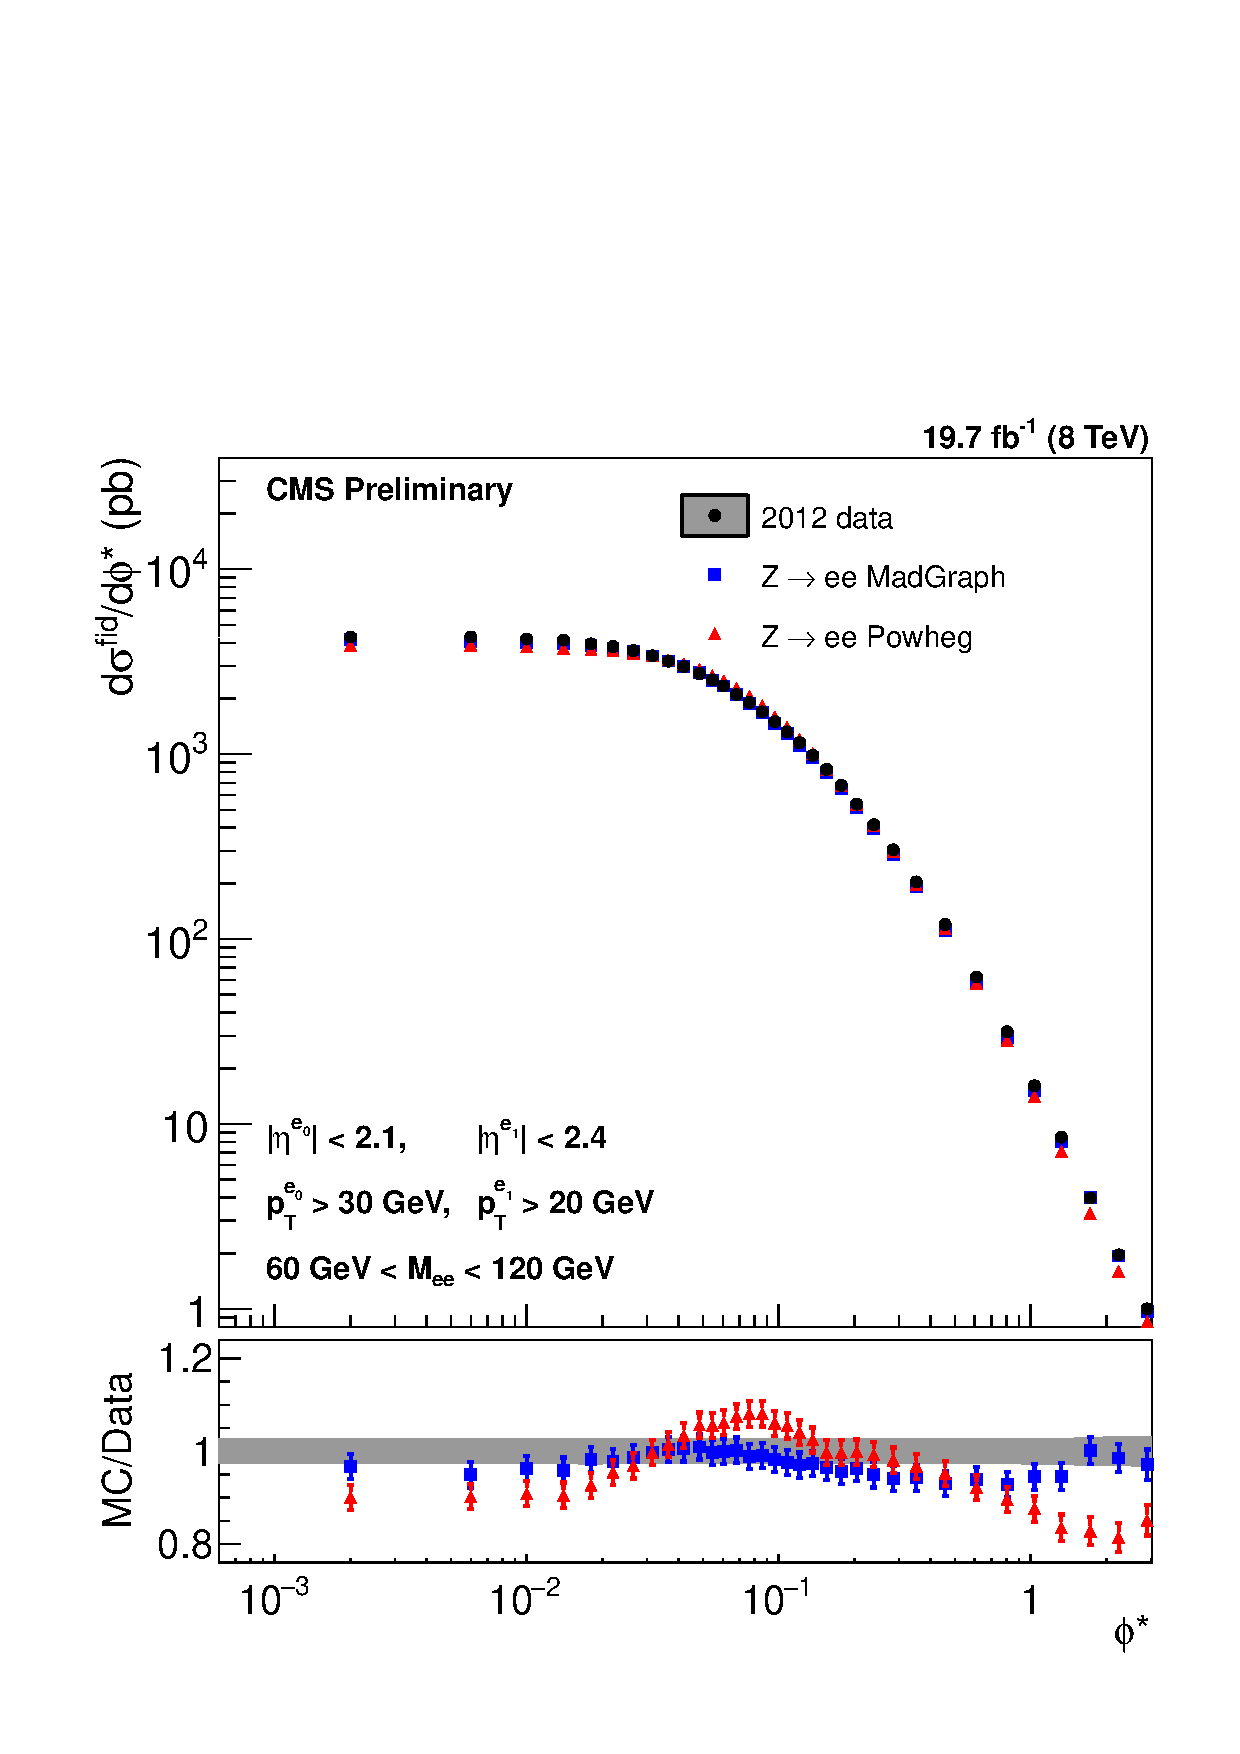
\includegraphics[width=\textwidth]{figures/ZShape_elec_Abs_Dressed.pdf}
    \caption[
        The absolute differential cross section with respects to \phistar for
        \Ztoee events in our fiducial region from data unfolded with \MADGRAPH,
        and the same distributions in \MADGRAPH and \POWHEG.
    ]{
        The absolute differential cross section with respects to \phistar for
        \Ztoee events in our fiducial region from data unfolded with \MADGRAPH,
        and the same distributions in \MADGRAPH and \POWHEG. A close up of the
        lower plot is shown in \cref{fig:results_ratio_abs}.
    }
    \label{fig:results_abs}
\end{figure}

\begin{figure}[!p]
    \centering
    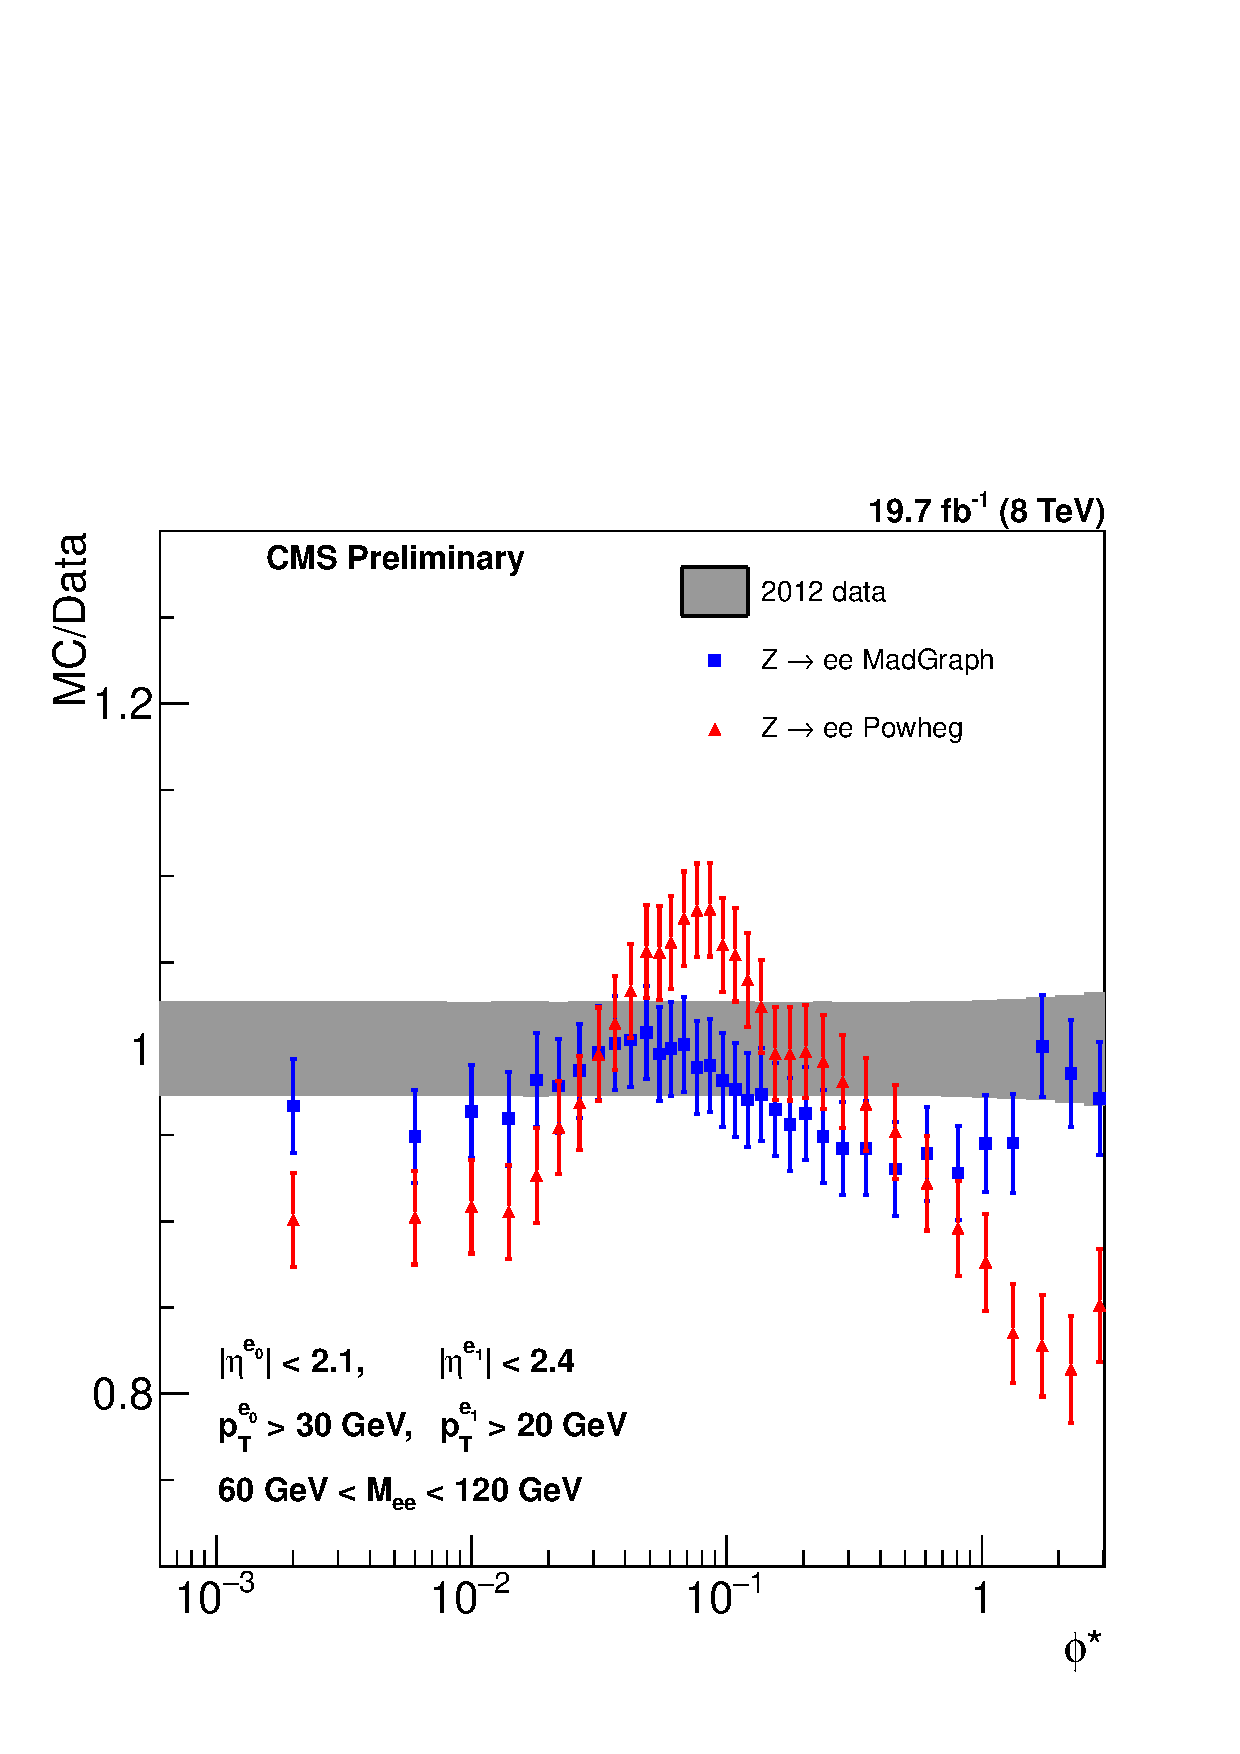
\includegraphics[width=\textwidth]{figures/ZShape_Ratioelec_Abs_Dressed.pdf}
    \caption[
        Close up of the ratio plot from \cref{fig:results_abs} for the
        absolute cross section measurement unfolded with \MADGRAPH.
    ]{
        Close up of the ratio plot from \cref{fig:results_abs} for the
        absolute cross section measurement unfolded with \MADGRAPH. The error
        band indicates the uncertainty in the data, while the square points
        show the ratio of \MADGRAPH over data, and the triangle points show the
        ratio of \POWHEG over data.
    }
    \label{fig:results_ratio_abs}
\end{figure}

% tab:results_abs
\begin{table}
    \spacerows{1.05}
    \begin{center}
        \begin{tabular}{@{}l r r r@{}}
            \toprule
            \phistar range & Data $(\pb)$ & \MADGRAPH $(\pb)$ & \POWHEG $(\pm)$ \\
            \midrule
            0.000--0.004  &  $4297  \pm  117$   &  $4155  \pm  138$   &  $3871  \pm  105$   \\
            0.004--0.008  &  $4302  \pm  117$   &  $4083  \pm  136$   &  $3881  \pm  105$   \\
            0.008--0.012  &  $4190  \pm  113$   &  $4037  \pm  134$   &  $3806  \pm  102$   \\
            0.012--0.016  &  $4137  \pm  113$   &  $3969  \pm  132$   &  $3746  \pm  103$   \\
            0.016--0.020  &  $3951  \pm  109$   &  $3879  \pm  129$   &  $3660  \pm  99$    \\
            0.020--0.024  &  $3816  \pm  103$   &  $3734  \pm  124$   &  $3642  \pm  100$   \\
            0.024--0.029  &  $3632  \pm  99$    &  $3586  \pm  119$   &  $3518  \pm  96$    \\
            0.029--0.034  &  $3404  \pm  93$    &  $3396  \pm  113$   &  $3393  \pm  92$    \\
            0.034--0.039  &  $3182  \pm  87$    &  $3192  \pm  106$   &  $3229  \pm  88$    \\
            0.039--0.045  &  $2971  \pm  81$    &  $2987  \pm  99$    &  $3071  \pm  83$    \\
            0.045--0.052  &  $2724  \pm  74$    &  $2750  \pm  91$    &  $2878  \pm  78$    \\
            0.052--0.057  &  $2521  \pm  69$    &  $2514  \pm  84$    &  $2662  \pm  73$    \\
            0.057--0.064  &  $2335  \pm  63$    &  $2335  \pm  78$    &  $2479  \pm  68$    \\
            0.064--0.072  &  $2099  \pm  57$    &  $2104  \pm  70$    &  $2257  \pm  62$    \\
            0.072--0.081  &  $1904  \pm  52$    &  $1883  \pm  63$    &  $2057  \pm  56$    \\
            0.081--0.091  &  $1694  \pm  46$    &  $1678  \pm  56$    &  $1831  \pm  49$    \\
            0.091--0.102  &  $1498  \pm  41$    &  $1471  \pm  49$    &  $1589  \pm  44$    \\
            0.102--0.114  &  $1320  \pm  36$    &  $1288  \pm  43$    &  $1392  \pm  38$    \\
            0.114--0.128  &  $1152  \pm  31$    &  $1118  \pm  37$    &  $1198  \pm  33$    \\
            0.128--0.145  &  $984   \pm  27$    &  $958   \pm  32$    &  $1008  \pm  27$    \\
            0.145--0.165  &  $827   \pm  22$    &  $797   \pm  27$    &  $824   \pm  22$    \\
            0.165--0.189  &  $678   \pm  18$    &  $648   \pm  22$    &  $676   \pm  18$    \\
            0.189--0.219  &  $537   \pm  15$    &  $517   \pm  17$    &  $536   \pm  15$    \\
            0.219--0.258  &  $415   \pm  11$    &  $394   \pm  13$    &  $412   \pm  11$    \\
            0.258--0.312  &  $304   \pm  8$     &  $287   \pm  10$    &  $298   \pm  8$     \\
            0.312--0.391  &  $204   \pm  6$     &  $192   \pm  6$     &  $197   \pm  5$     \\
            0.391--0.524  &  $120   \pm  3$     &  $112   \pm  4$     &  $114   \pm  3$     \\
            0.524--0.695  &  $62    \pm  2$     &  $59    \pm  2$     &  $58    \pm  2$     \\
            0.695--0.918  &  $31.6  \pm  0.9$   &  $29.3  \pm  1.0$   &  $28.3  \pm  0.7$   \\
            0.918--1.153  &  $16.1  \pm  0.5$   &  $15.2  \pm  0.5$   &  $14.1  \pm  0.4$   \\
            1.153--1.496  &  $8.5   \pm  0.2$   &  $8.0   \pm  0.3$   &  $7.1   \pm  0.2$   \\
            1.496--1.947  &  $4.0   \pm  0.1$   &  $4.0   \pm  0.1$   &  $3.3   \pm  0.1$   \\
            1.947--2.522  &  $1.96  \pm  0.06$  &  $1.93  \pm  0.07$  &  $1.60  \pm  0.06$  \\
            2.522--3.277  &  $1.00  \pm  0.03$  &  $0.97  \pm  0.03$  &  $0.85  \pm  0.03$  \\
            \bottomrule
        \end{tabular}
    \end{center}
    \caption[
        Differential cross-section in \pb with respect to \phistar of \Ztoee.
    ]{
        Differential cross-section in \pb with respect to \phistar of \Ztoee in
        our fiducial region in data and as generated by \MADGRAPH and \POWHEG.
        These results are shown graphically in figure~\ref{fig:result_abs}.
    }
    \label{tab:results_abs}
\end{table}


The absolute differential cross section measurement using data unfolded with
\POWHEG is shown in \FIG~\ref{fig:results_abs_powheg} and given in tabular form
in \TAB~\ref{tab:results_abs_powheg}. The lower plot in
\FIG~\ref{fig:results_abs_powheg} is shown in more detail in
\FIG~\ref{fig:results_ratio_abs_powheg}. The primary uncertainty on the data
distribution is still from the integrated luminosity, although the MC
statistical uncertainty is larger in the highest \phistar bins.

% fig:results_abs_powheg and fig:results_ratio_abs_powheg
\begin{figure}[!p]
    \centering
    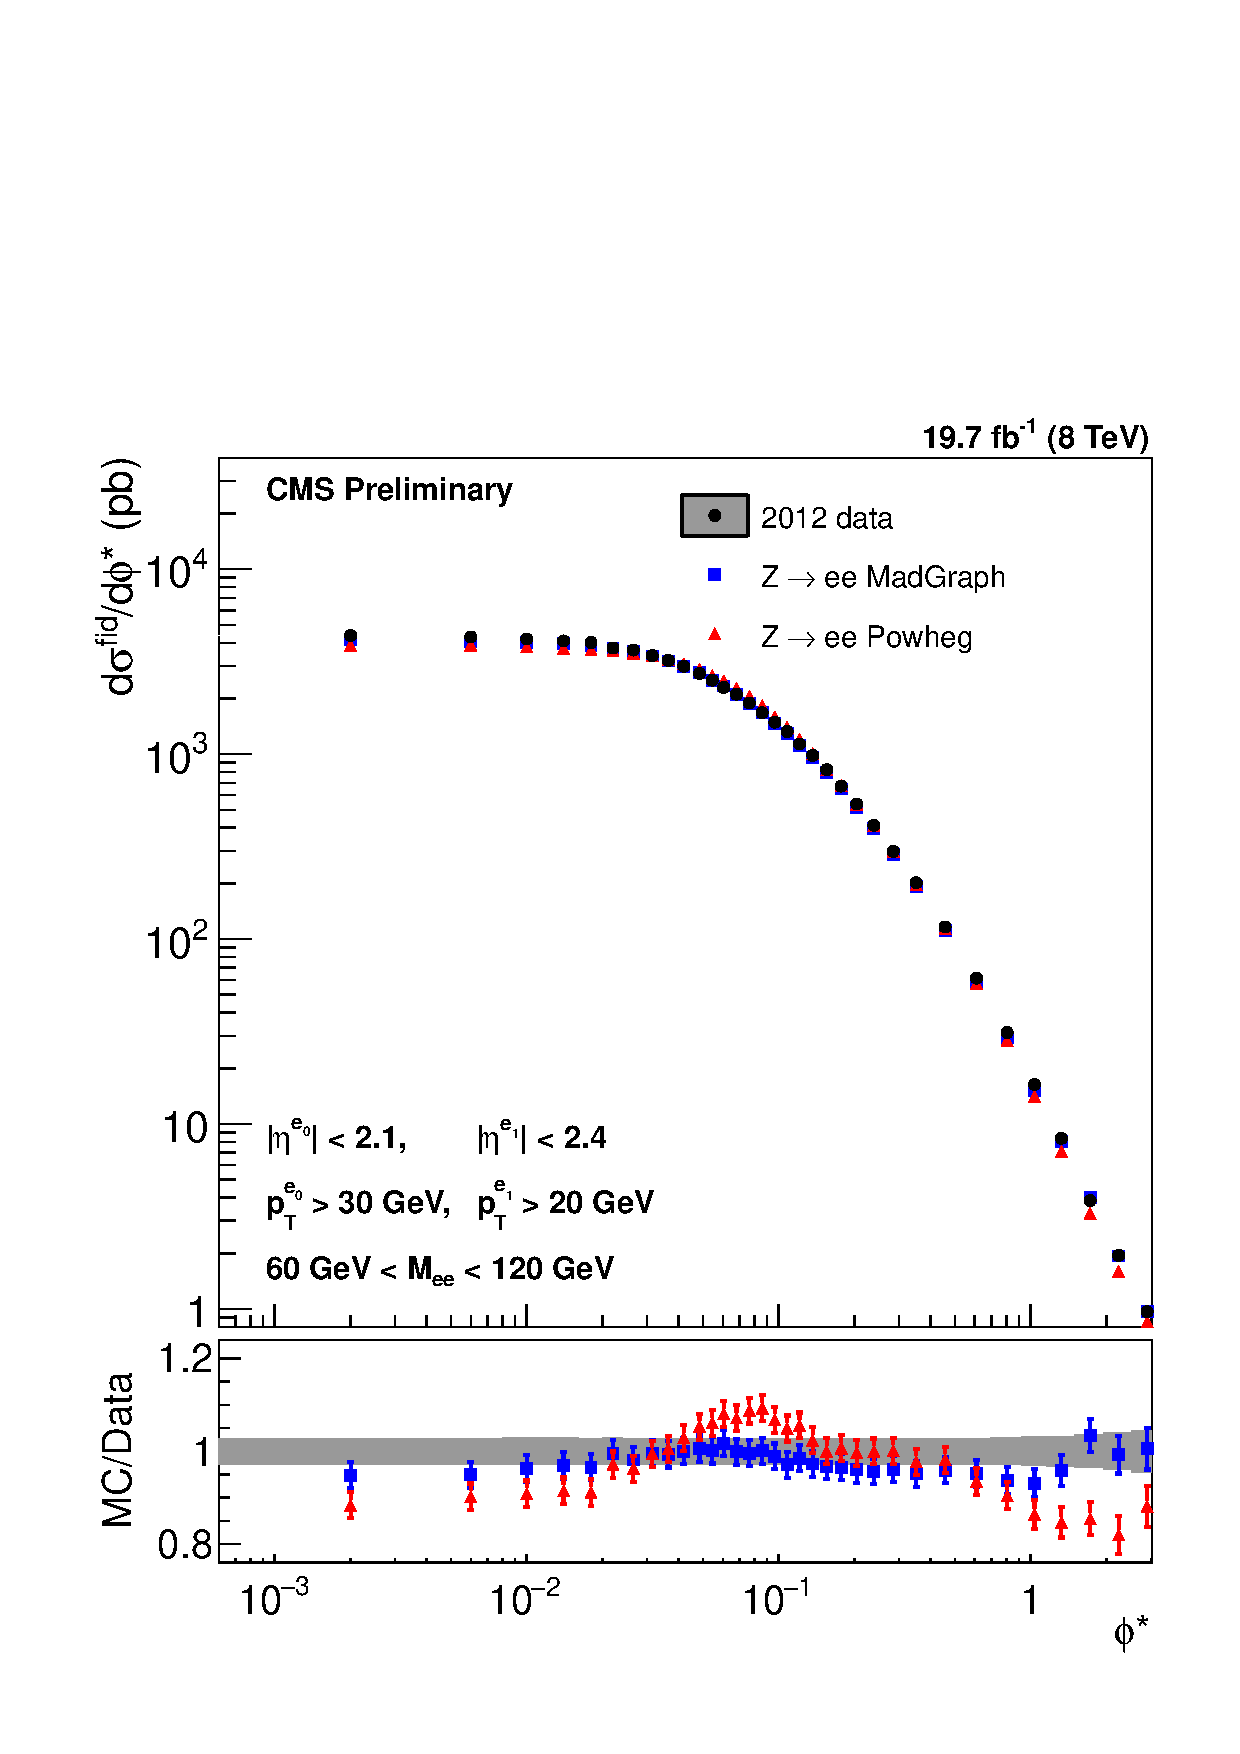
\includegraphics[width=\textwidth]{figures/ZShape_elec_PH_Abs_Dressed.pdf}
    \caption[
        The absolute differential cross section with respects to \phistar for
        \Ztoee events in our fiducial region from data unfolded with
        \PPsixZtwo.
    ]{
        The absolute differential cross section with respects to \phistar for
        \Ztoee events in our fiducial region from data unfolded with
        \PPsixZtwo, and the same distributions in \MADGRAPH and \PPsixZtwo. A
        close up of the lower plot is shown in
        \cref{fig:results_ratio_abs_powheg}.
    }
    \label{fig:results_abs_powheg}
\end{figure}

\begin{figure}[!p]
    \centering
    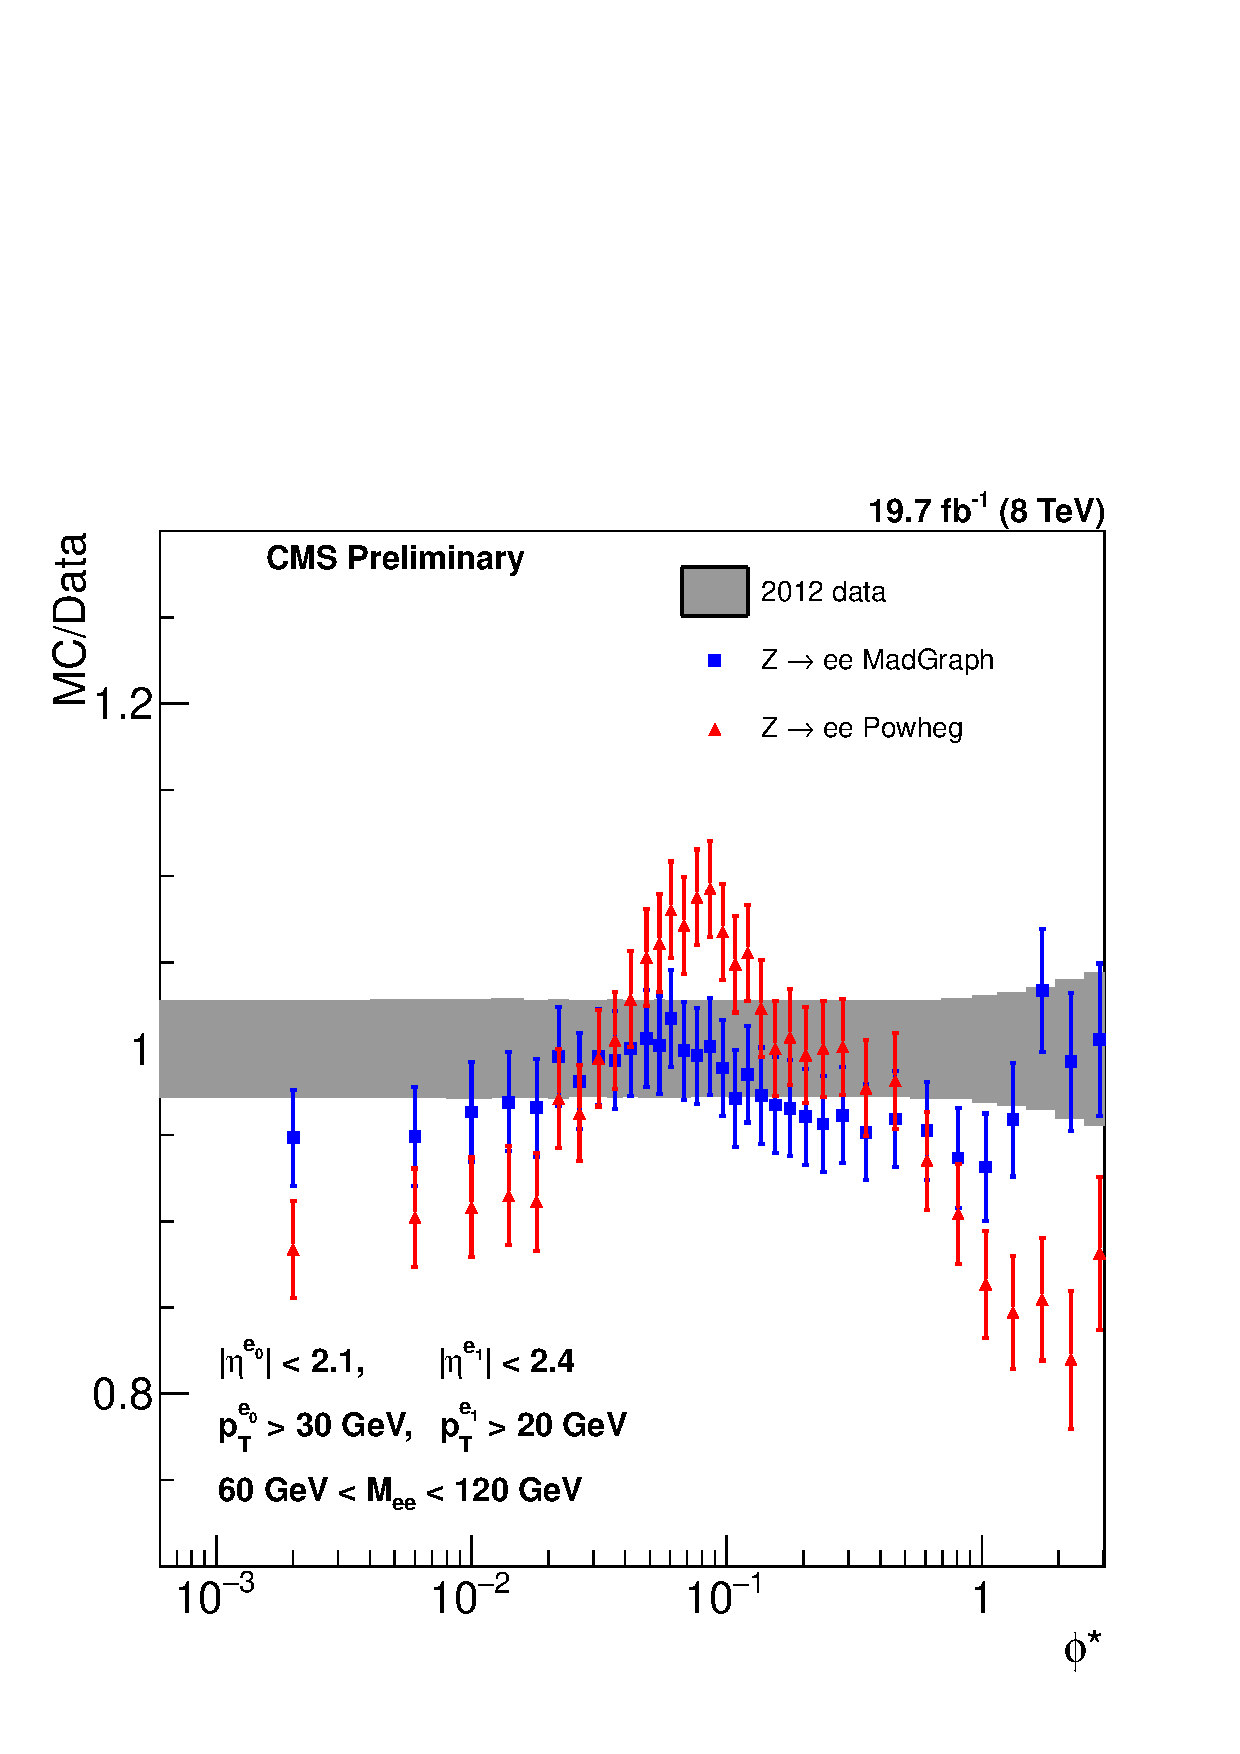
\includegraphics[width=\textwidth]{figures/ZShape_Ratioelec_PH_Abs_Dressed.pdf}
    \caption[
        Close up of the ratio plot from \cref{fig:results_abs_powheg} for the
        absolute cross section measurement unfolded with \PPsixZtwo.
    ]{
        Close up of the ratio plot from \cref{fig:results_abs_powheg} for the
        absolute cross section measurement unfolded with \PPsixZtwo. The error
        band indicates the uncertainty in the data, while the square points
        show the ratio of \MADGRAPH over data, and the triangle points show the
        ratio of \PPsixZtwo over data.
    }
    \label{fig:results_ratio_abs_powheg}
\end{figure}

% tab:results_abs_powheg
\begin{table}
    \spacerows{1.05}
    \begin{center}
        \begin{tabular}{@{}l r r r@{}}
            \toprule
            \phistar range & Data $(\pb)$ & \MADGRAPH $(\pb)$ & \POWHEG $(\pm)$ \\
            \midrule
            0.000--0.004  &  $4381  \pm  122$   &  $4155  \pm  138$   &  $3871  \pm  105$   \\
            0.004--0.008  &  $4302  \pm  122$   &  $4083  \pm  136$   &  $3881  \pm  105$   \\
            0.008--0.012  &  $4191  \pm  121$   &  $4037  \pm  134$   &  $3806  \pm  102$   \\
            0.012--0.016  &  $4096  \pm  118$   &  $3969  \pm  132$   &  $3746  \pm  103$   \\
            0.016--0.020  &  $4016  \pm  113$   &  $3879  \pm  129$   &  $3660  \pm  99$    \\
            0.020--0.024  &  $3751  \pm  108$   &  $3734  \pm  124$   &  $3642  \pm  100$   \\
            0.024--0.029  &  $3654  \pm  102$   &  $3586  \pm  119$   &  $3518  \pm  96$    \\
            0.029--0.034  &  $3412  \pm  95$    &  $3396  \pm  113$   &  $3393  \pm  92$    \\
            0.034--0.039  &  $3213  \pm  91$    &  $3192  \pm  106$   &  $3229  \pm  88$    \\
            0.039--0.045  &  $2985  \pm  83$    &  $2987  \pm  99$    &  $3071  \pm  83$    \\
            0.045--0.052  &  $2734  \pm  77$    &  $2750  \pm  91$    &  $2878  \pm  78$    \\
            0.052--0.057  &  $2509  \pm  71$    &  $2514  \pm  84$    &  $2662  \pm  73$    \\
            0.057--0.064  &  $2295  \pm  65$    &  $2335  \pm  78$    &  $2479  \pm  68$    \\
            0.064--0.072  &  $2107  \pm  59$    &  $2104  \pm  70$    &  $2257  \pm  62$    \\
            0.072--0.081  &  $1891  \pm  53$    &  $1883  \pm  63$    &  $2057  \pm  56$    \\
            0.081--0.091  &  $1676  \pm  47$    &  $1678  \pm  56$    &  $1831  \pm  49$    \\
            0.091--0.102  &  $1488  \pm  41$    &  $1471  \pm  49$    &  $1589  \pm  44$    \\
            0.102--0.114  &  $1327  \pm  37$    &  $1288  \pm  43$    &  $1392  \pm  38$    \\
            0.114--0.128  &  $1135  \pm  32$    &  $1118  \pm  37$    &  $1198  \pm  33$    \\
            0.128--0.145  &  $985   \pm  28$    &  $958   \pm  32$    &  $1008  \pm  27$    \\
            0.145--0.165  &  $824   \pm  23$    &  $797   \pm  27$    &  $824   \pm  22$    \\
            0.165--0.189  &  $671   \pm  19$    &  $648   \pm  22$    &  $676   \pm  18$    \\
            0.189--0.219  &  $538   \pm  15$    &  $517   \pm  17$    &  $536   \pm  15$    \\
            0.219--0.258  &  $412   \pm  11$    &  $394   \pm  13$    &  $412   \pm  11$    \\
            0.258--0.312  &  $298   \pm  8$     &  $287   \pm  10$    &  $298   \pm  8$     \\
            0.312--0.391  &  $202   \pm  6$     &  $192   \pm  6$     &  $197   \pm  5$     \\
            0.391--0.524  &  $116   \pm  3$     &  $112   \pm  4$     &  $114   \pm  3$     \\
            0.524--0.695  &  $61    \pm  2$     &  $59    \pm  2$     &  $58    \pm  2$     \\
            0.695--0.918  &  $31.3  \pm  0.9$   &  $29.3  \pm  1.0$   &  $28.3  \pm  0.7$   \\
            0.918--1.153  &  $16.4  \pm  0.5$   &  $15.2  \pm  0.5$   &  $14.1  \pm  0.4$   \\
            1.153--1.496  &  $8.4   \pm  0.3$   &  $8.0   \pm  0.3$   &  $7.1   \pm  0.2$   \\
            1.496--1.947  &  $3.9   \pm  0.1$   &  $4.0   \pm  0.1$   &  $3.3   \pm  0.1$   \\
            1.947--2.522  &  $1.95  \pm  0.08$  &  $1.93  \pm  0.07$  &  $1.60  \pm  0.06$  \\
            2.522--3.277  &  $0.97  \pm  0.04$  &  $0.97  \pm  0.03$  &  $0.85  \pm  0.03$  \\
            \bottomrule
        \end{tabular}
    \end{center}
    \caption[
        The absolute differential cross section in \pb with respects to
        \phistar for \Ztoee events in our fiducial region from data unfolded
        with \POWHEG.
    ]{
        The absolute differential cross section in \pb with respects to
        \phistar for \Ztoee events in our fiducial region from data unfolded
        with \POWHEG, and the same distributions in \MADGRAPH and \POWHEG.
        These results are shown graphically in
        figure~\ref{fig:results_abs_powheg}.
    }
    \label{tab:results_abs_powheg}
\end{table}

